\documentclass[b5paper]{report}
\usepackage[lmargin=25mm,rmargin=25mm,tmargin=27mm,bmargin=30mm]{geometry}
\usepackage{color}
\usepackage{xcolor}
\usepackage{tikz}
\usepackage{pgfplots}
\usepackage{graphicx}
\usepackage{wrapfig}
\usepackage{svg}
\usepackage{float}
\usepackage{url}
\usepackage{parskip}
\usepackage[chapter]{minted}

\graphicspath{{images/}}
\svgpath{{images/}}
\usetikzlibrary{positioning}
\usetikzlibrary{shapes,decorations,shadows}

\begin{document}
\title{Efficient recovery in a data-flow based storage system}
\author{Martin Ek}
\date{\today}
\maketitle

\newcommand{\note}[1]{{\color{olive}\sffamily #1}}
\newcommand{\todo}[1]{{\color{purple}\sffamily[TODO: #1]}}
\newcommand{\eg}{\textit{e.g.},\xspace}
\newcommand{\ie}{\textit{i.e.},\xspace}
\newcommand{\vs}{\textit{vs.}\xspace}
\newcommand{\viz}{\textit{viz.},\xspace}

% Handy superscript macros
\newcommand{\stss}{\textsuperscript{st}}
\newcommand{\ndss}{\textsuperscript{nd}}
\newcommand{\rdss}{\textsuperscript{rd}}
\newcommand{\thss}{\textsuperscript{th}}

% Enumeration commands
\newcommand{\one}{({\em i}\/)}
\newcommand{\two}{({\em ii}\/)}
\newcommand{\three}{({\em iii}\/)}
\newcommand{\four}{({\em iv}\/)}
\newcommand{\five}{({\em v}\/)}

\newcommand\code[1]{\texttt{#1}}


\begin{abstract}
  Growing performance demands in today's web applications have lead to developers
  introducing complex cache hierarchies to deal with poor read performance in
  traditional database systems. Soup is a new and highly scalable database system
  that sets out to remove the need for these caching solutions, providing
  impressive read performance right out of the box even for complex queries,
  without the downsides of having to manually invalidate cached data.

  Soup achieves this by building up and maintaining a data-flow graph, avoiding
  the need to manually maintain materialized views. By adapting the graph to
  schema changes on-the-fly, Soup avoids the substantial downtime that
  comes with migrations in traditional relational database management systems.

  Utilizing a group-commit protocol, Soup persists all base table writes to a
  log on durable storage before propagating changes throughout the graph.
  Recovery is based on replaying the semantic updates from its logs, which
  naturally leads to gradually increasing recovery times as a database acquires
  more data. Checkpointing by taking a snapshot of the database's current state
  is a common way to solve this issue, reducing the size of the log at the same
  time. This is not trivial in Soup however, where the data is spread across
  materializations in the data-flow graph, and updates are propagated through
  the graph asynchronously without timestamps.

  This thesis approaches the problem of creating a logically consistent snapshot
  across Soup's data-flow graph by utilizing snapshotting techniques common in
  distributed systems, considering each node in Soup's query graph as a single
  node in a distributed setting. Initial results are promising, and shows an
  overall reduction in recovery time of 90\% compared to log based recovery,
  without a significant impact on the running system's write throughput.
\end{abstract}

\tableofcontents
\pagebreak

\chapter{Introduction}
Soup is developed at the Parallel and Distributed Operating System group at
MIT CSAIL \cite{soup-web}. The latest prototype of the system is implemented using
the Rust programming language and is freely available with a permissive license
on GitHub \cite{distributary}.

Chapter \ref{chap:background} introduces Soup as a system, together with a few
commonly utilized techniques for recovery in main-memory databases and a brief
introduction to the Rust programming language. Chapter \ref{chap:methodology}
presents the implemented solution for log based recovery, followed by gradually
building up a snapshotting algorithm compatible with Soup. This algorithm is
then implemented, and its performance is inspected in chapter
\ref{chap:results}.

Finally, chapter \ref{chap:discussion} looks at a few possible areas for
improvement, while drawing conclusions regarding the covered recovery methods.

\chapter{Background} \label{chap:background}
\section{Soup}
Modern web applications face an increasingly difficult performance problem in
relation to their storage needs: traditional relational databases perform too
poorly when used in isolation. Either by failing to scale to a large amount of
concurrent users, or by taking too long to return results for more expensive
aggregation queries.

This is often worked around by building up intricate cache hierarchies
\cite{memcached}, similar to the multi-level cache hierarchy readers might be
accustomed to seeing in their processors. This solves both performance problems:
concurrent readers can access materialized data from the upper levels of the
cache hierarchy, achieving low latency and high throughput even when faced with
large amounts of clients. Expensive queries then only need to be performed once,
as long as the result is invalidated when the underlying data changes. Write
operations still need to change the underlying storage layer however, but are
now also responsible for clearing out or updating the materialized cache levels.

This adds an extra layer of complexity, and is a trade-off accepted by almost
every modern day developer that faces more than a trivial amount of load to
their storage system.

Soup sets out to solve this by providing a single high performing system,
removing the need for manual materialization altogether. The current prototype
scales to millions of writes and reads per second \cite{soup}, and works both on
a single machine and in a distributed setting.

\begin{figure}
  \centering
  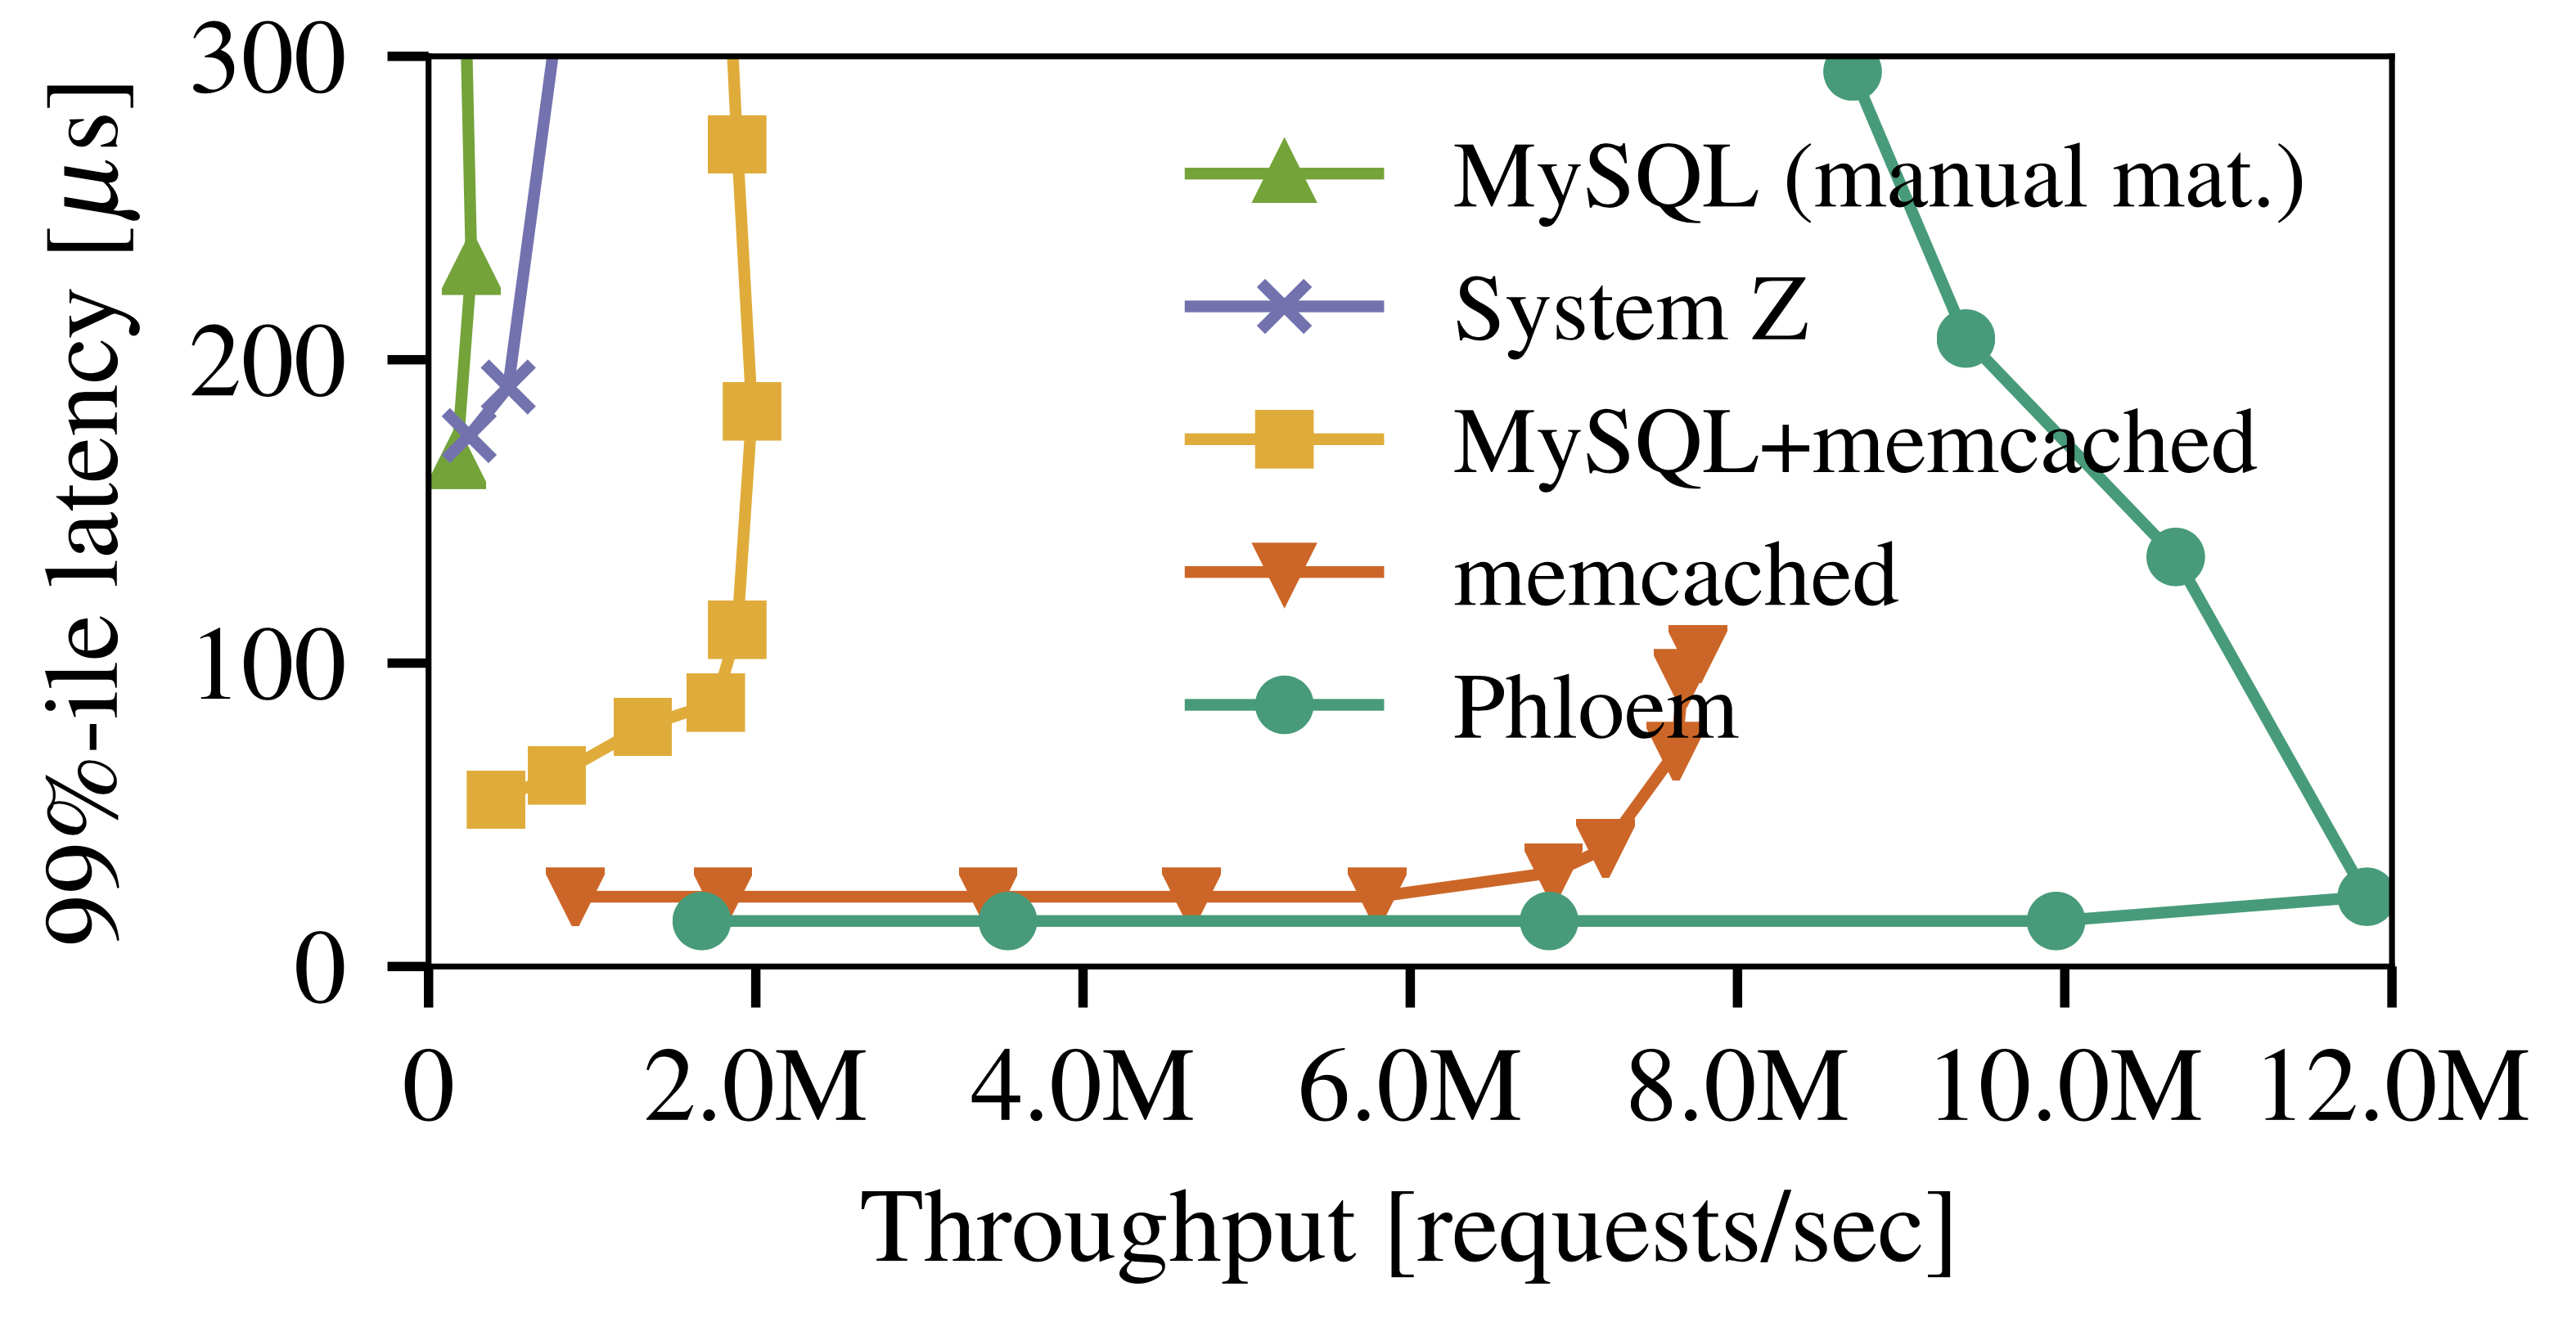
\includegraphics[width=\textwidth]{read}
  \caption{
    Soup (here: \textit{Phloem}) outperforms even the popular caching
    system memcached on read-heavy (95\% reads) workloads.
  }
\end{figure}

\begin{figure}
  \centering
  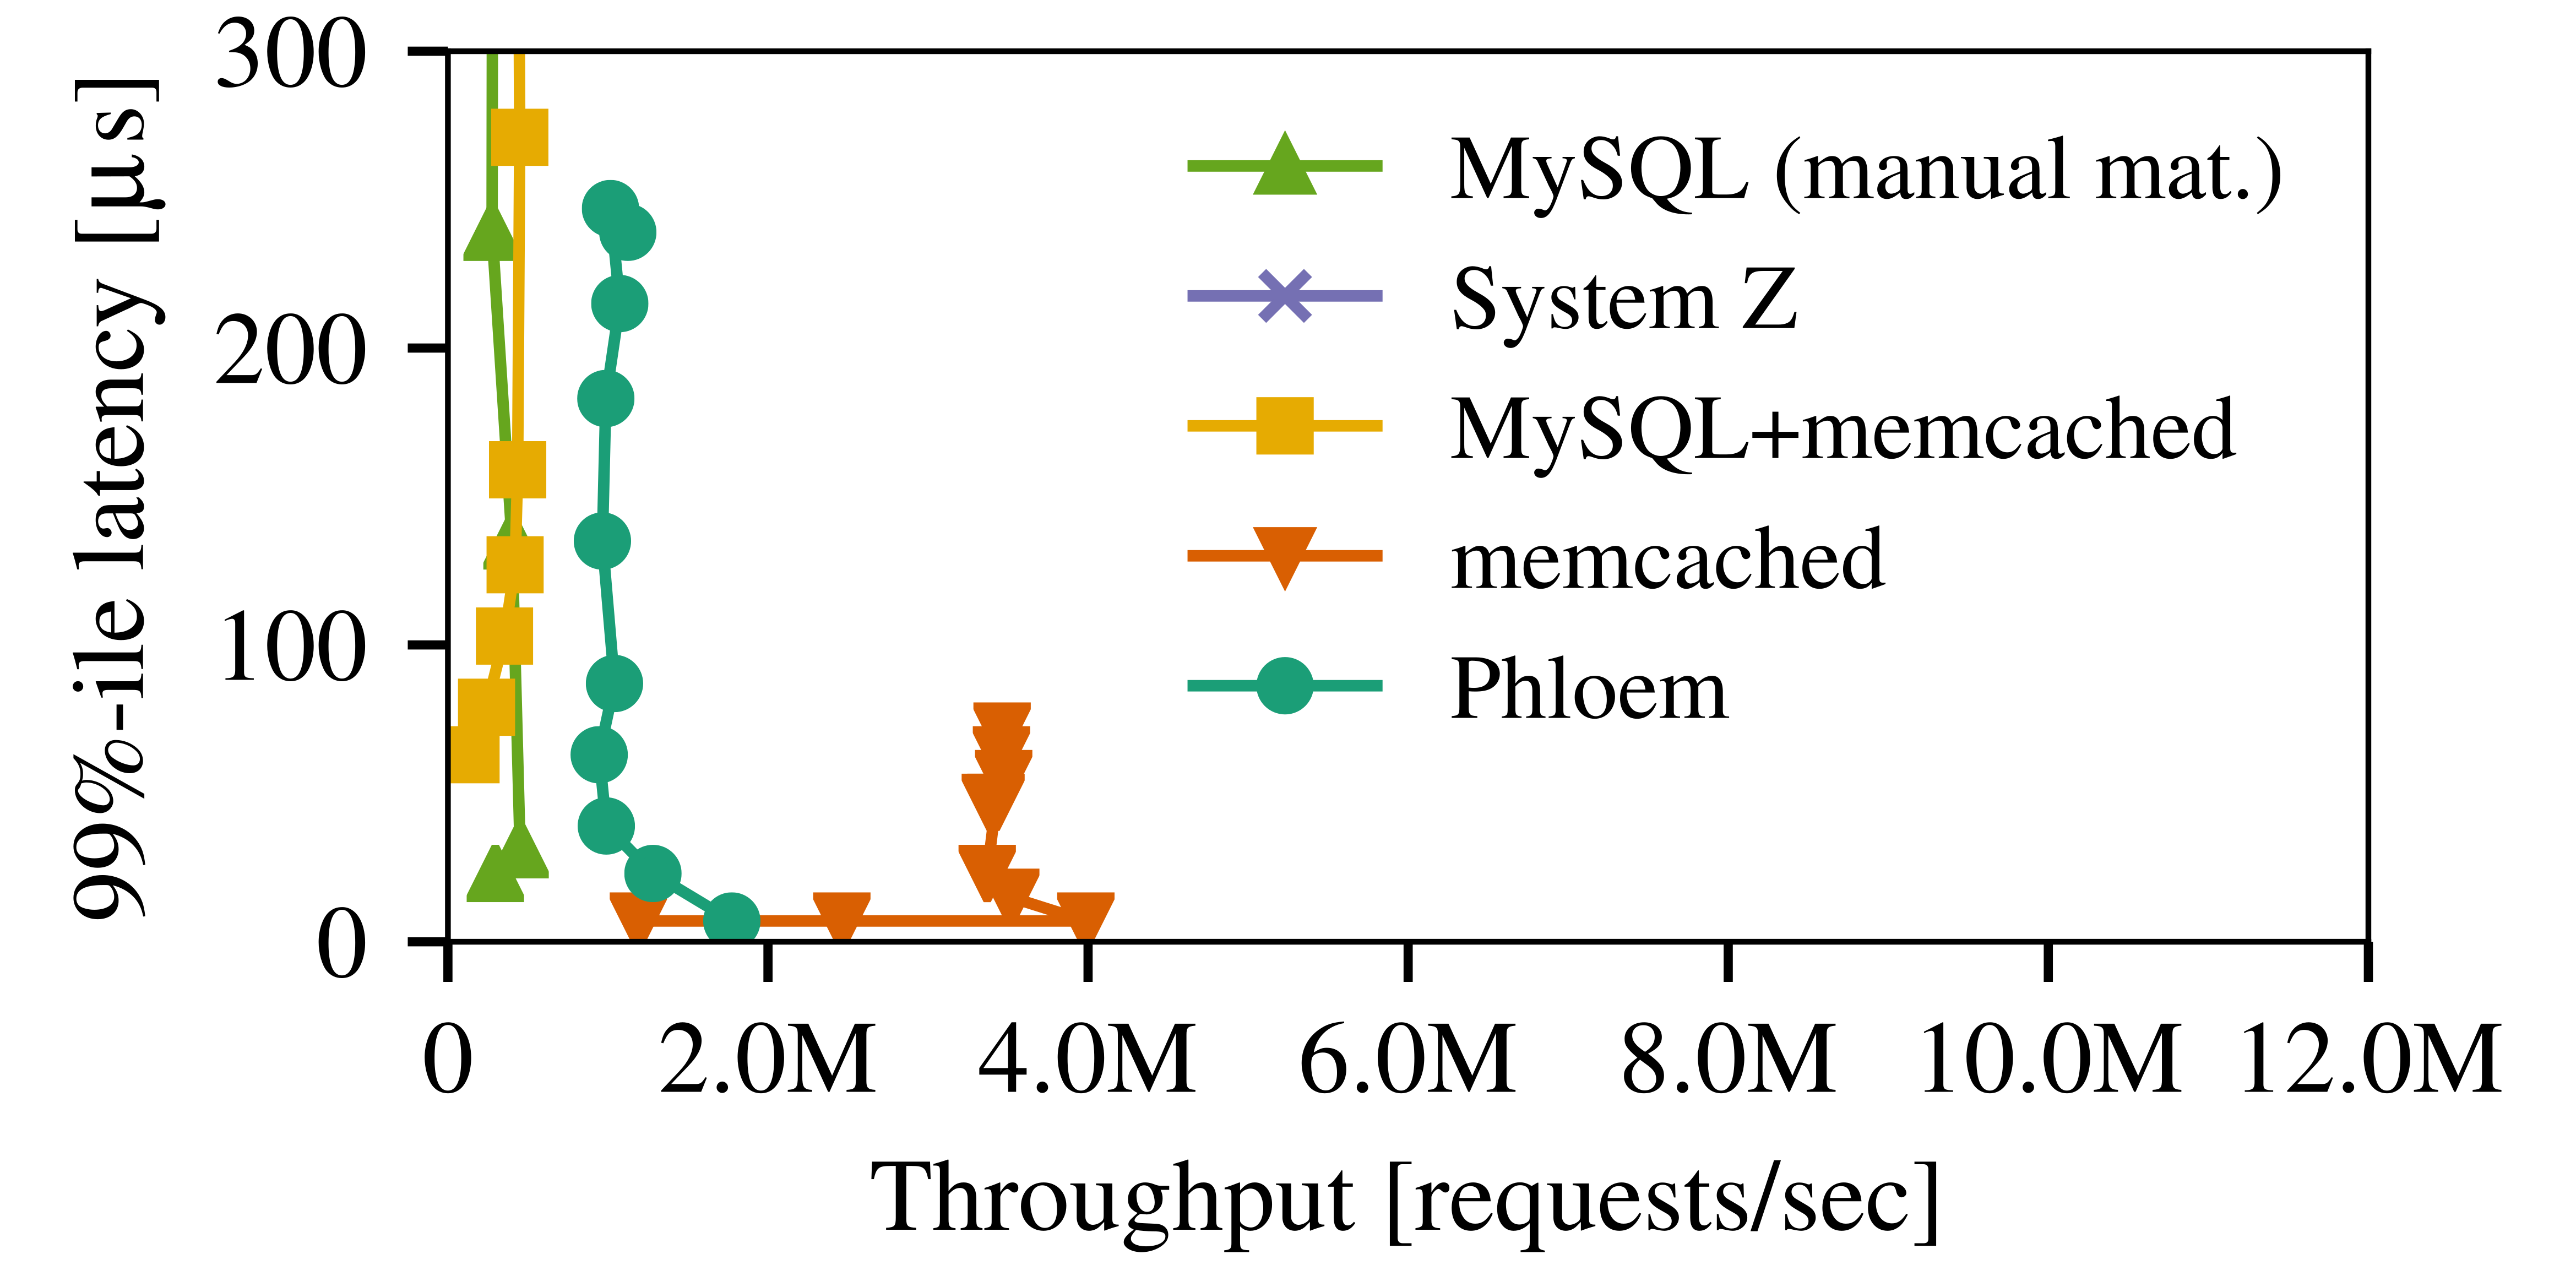
\includegraphics[width=\textwidth]{mixed}
  \caption{
    Soup (here: \textit{Phloem}) still holds up well when faced with a 50\%/50\%
    mixed read/write workload.
  }
\end{figure}

Soup does this by materializing data automatically in a data-flow
graph, building on existing streaming data-flow research \cite{naiad, dataflow}
by combining it with ideas from performant materialized view solutions
\cite{dbtoaster, pequod}.

\subsection{Data-flow Graph}
Soup turns base table schemas and a pre-defined list of queries into a data-flow
graph that doubles as a set of materialized views. The base tables form the
root nodes of the graph, and all writes propagate from here. The graph itself
resembles the query graph of a traditional relational database system
\cite{codd}, with the graph's intermediate nodes being relational operators.

However, whereas a relational database management system's query graph is used
primarily to retrieve data, by executing operators to fetch data from durable
storage, Soup's graph does the exact opposite. The graph is defined ahead of
queries being received, and writes stream through the relevant nodes in the
graph - starting from the base nodes. This skews the majority of the system's
work towards writes, as results are materialized at different nodes throughout
the graph.

The query graph includes at least one materialized node per pre-defined query,
located at the bottom of the graph as leaf nodes. This means that reading from
the system is a matter of finding the relevant leaf node, and retrieving data
from the node's materialized storage. This is one of the elements that makes Soup
resemble more of a key-value store than a traditional RDBMS. Even though Soup
supports advanced SQL queries, both mutations and retrievals are done with a
key, which then maps to a corresponding value.

On an elementary level one could see Soup creating a separate graph for each
query, similar to query graphs in traditional database systems, but that would
have been quite inefficient. For one it would have lead to Soup materializing a
lot of duplicate data for intermediary materialized nodes, and base table writes
would have had to be propagated to more nodes than necessary. Migrations would
also have taken considerably longer time, as adding queries would mean
constructing a completely new query graph. Instead Soup uses multi-query
optimization techniques to create common sub-graphs of nodes that can be used in
multiple queries.

\subsubsection{Domains}
Soup's data-flow graph is divided into logical domains, where each domain
contains a series of nodes. Within a domain, a single update is processed at a
time, removing the need for internal locks. Each domain is separated into a
different computational entity, either a thread, or a separate Soup client when
the system is run in a distributed fashion.

Domains are separated by ingress and egress nodes, where a boundary between
these are formed on the form of a buffered channel. In a multi-machine Soup
setup, the ingress and egress nodes are connected with TCP connections instead.

Note that domains do not handle read operations. These are served directly from
the leaf nodes by separate worker threads, maintaining high read performance
even in the midst of processing a large amount of writes.

\subsection{Architecture}
At the core of a running Soup system is the controller, which serves as the
initial entry point for communication with the rest of the Soup system. Clients
communicate with the controller over a TCP-based remote procedure call (RPC)
interface, exposing a series of building blocks that open for interaction with
the database. Two of the most central parts here are mutators and getters, which
allow respectively writing and reading from the data-flow graph. After getting a
hold of a mutator, clients perform writes and reads without going through the
controller. While this avoids the controller becoming a performance bottleneck,
the argument that the controller corresponds to a single failure point for a
distributed Soup still holds. The latest version of Soup improves this by making
controllers fault-tolerant, using ZooKeeper \cite{zookeeper} to implement
consensus.

\subsubsection{Souplets}
The actual work performed by a Soup system is done in Souplets, which
correspond to separate instances that communicate in a distributed fashion. Each
Souplet has a pool of workers, where domains are spread throughout the pool.
Previous implementations of Soup ran each domain in its own separate thread,
which led to reduced performance when the amount of domains went up in
core-constrained systems. A worker pool solves this by setting a cap on the
amount of threads that process domains, such that a single thread might be
responsible for processing packets for multiple domains.

Soup also supports running completely in one process, which is convenient for
local development and testing. In that case there is only a single worker pool,
which the controller is responsible for starting.

Communication between the Souplet instances and the controller is done over TCP,
in a layer that is referred to as the coordination plane. This involves
heartbeat messages, but also packets that are sent when domains are assigned,
re-assigned and removed to different Souplet instances.

\subsubsection{Backlog} \label{sec:readers}
Data written through mutators are sent through the data-flow graph, where they
eventually reach the leaf nodes: the readers. Here data is persisted into an
in-memory eventually consistent data structure, an \texttt{evmap} \cite{evmap}.
Getters then expose the records residing here by accessing the readers directly,
avoiding the need to go through the entire graph to retrieve data.
\texttt{evmap} implements reading without any locks at all, avoiding degrading
performance for read-heavy work loads.

\subsection{Materialization} \label{sec:materialization}
Similar to traditional relational databases, writes are inserted into the
table directly - a base node in Soup. Whereas this marks the end of the
operation for an RDBMS, Soup will continue by propagating the write throughout
the query graph, storing the result at materialized nodes.

The insertions are handled with a group-commit protocol, where records are
batched up and finally inserted into a durable log before being propagated to
the base node.

Soup primarily materializes leaf nodes in the graph, to enable fast read
queries. In some cases intermediary operators might also choose to materialize
the records they receive before they forward them through to their child nodes.
This is especially the case for stateful operators, such as extremum queries, as
these need to incrementally update their result - instead of having to go
through and re-calculate the state on every new record.

Nodes can also be partially materialized, which lets each node choose which rows
to keep in their internal state. This resembles a regular caching system, where
keys can be evicted after a period of inactivity.

\subsection{Migrations}
Relational databases require developers to pre-define a set of table schemas for
their application. Changes to these throughout a project's life cycle are often
inevitable, however the process of performing migrations in a live
system without downtime is usually far from trivial \cite{stripe}. This is one
of the core issues Soup sets out to solve, by providing a database system that
lets developers change both the base table schemas and the pre-defined queries
at any point.

Soup constructs a new graph for added queries. This is done by finding overlaps
with the existing query graph nodes, to avoid duplicate materializations and
to reduce the amount of work done by each migration. Soup marks nodes as
partially materialized when possible, which lets the system start processing
requests for the newly defined query right away, by only fetching each key from
ancestor nodes when necessary. For fully materialized nodes, Soup will replay
all relevant base table writes from the closest materialized node. This
delays the point where Soup can start processing requests, but has the advantage
of not delaying subsequent requests to retrieve materialized keys later on.

Modifications to base table schemas are done in-place, by having Soup's base
nodes internally include the full history of columns for that specific table.
% TODO: default values

\subsection{Transactions}
An increasing amount of real-world database system users have found relaxed
consistency guarantees to be sufficient in the last few years, as it greatly
simplifies the problem of replicating large amounts of data across data centers
with high performance \cite{existential}. There are nonetheless without doubt
a wide variety of use cases for transactions, where the eventual consistency that
Soup offers is insufficient. To cater to these types of applications, Soup
allows developers to opt-in for transaction support, by defining their base
nodes as transactional.

Soup's transaction support is carefully designed to avoid slowing down
non-transactional workloads. Using optimistic concurrency control, Soup returns
timestamped tokens for reads, which can later be used to verify the validity of
the data that was read. Writes can only be performed at the end of a
transaction, when clients request their transactions to be committed. The
timestamp part of the token helps Soup validate if concurrent clients
interfered with the data, which lets the system notify the client by aborting
the ongoing transaction.

\subsection{Example} \label{example}
Having presented the different parts of the Soup system, lets look at how using
Soup currently works. The example in listing \ref{lst:soup-example} builds up a query
graph from scratch, then performs a few simple writes and reads to the running
instance.

The example simulates users voting on a series of different articles, and
includes two base tables: \texttt{Article} and \texttt{Vote}. It highlights the
use of two types of queries: internal and external. The former can be seen as a
helper for the latter, where only external queries are exposed to the user. The
output query in the example counts the number of votes for a specific article,
through a \texttt{JOIN} between the two tables.

\begin{listing}[H]
  \begin{minted}[frame=lines, linenos]{rust}
let sql = "
    # Base tables:
    CREATE TABLE Article (aid int, title varchar(255), \
                         url text, PRIMARY KEY(aid));
    CREATE TABLE Vote (aid int, uid int);

    # Internal query:
    VoteCount: SELECT Vote.aid, COUNT(uid) AS votes \
                FROM Vote GROUP BY Vote.aid;

    # External query (note the QUERY keyword):
    QUERY ArticleWithVoteCount: \
                SELECT Article.aid, title, url, VoteCount.votes AS votes \
                FROM Article, VoteCount \
                WHERE Article.aid = VoteCount.aid AND Article.aid = ?;";

// set up Soup via recipe
let mut blender = ControllerBuilder::default().build();
blender.install_recipe(sql.to_owned());

// Build the mutators and the getter:
let inputs = blender.inputs();
let outputs = blender.outputs();
let mut article_mutator = blender.get_mutator(inputs["Article"]).unwrap();
let mut vote_mutator = blender.get_mutator(inputs["Vote"]).unwrap();
let mut count_getter = blender
  .get_getter(outputs["ArticleWithVoteCount"])
  .unwrap();

// Create a new article:
let aid = 1;
let title = "test title";
let url = "http://pdos.csail.mit.edu";
article
    .put(vec![aid.into(), title.into(), url.into()])
    .unwrap();

// Then create a vote:
let uid = 1;
vote.put(vec![aid.into(), uid.into()]).unwrap();

// Finally, retrieve the vote count:
// (the second argument states that we want to block until the result is ready)
println!("Vote Count: {:?}", vote_count.lookup(&aid.into(), true))
  \end{minted}
  \caption{
    Writing to and reading from a Soup instance.
    \label{lst:soup-example}
  }
\end{listing}

\section{Recovery} \label{aries}
At the core of most database systems you will find a log manager, which
maintains a sequence of log records on disk. Logging is essential in maintaining
fault tolerance and durability, and is used for a variety of issues: ensuring
the durability of committed data, recovering from failures, and rolling back
aborted transactions.

Even to this day one of the most popular algorithms for recovery is ARIES
\cite{aries} (Algorithm for Recovery and Isolation Exploitation Semantic), which
uses a write-ahead log to make sure that a persistent record of changes is
maintained before the actual changes themselves. Upon recovery ARIES makes sure
that all actions from the log prior to a crash are repeated (\textit{REDO}),
then reverts the operations belonging to failing transactions (\textit{UNDO}).
The former makes sure that durability is respected, while the latter maintains
atomicity.

Whereas the logging protocol used for recovery varies from implementation to
implementation, the principle behind a write-ahead log remains the same. By
maintaining a log of actions \textit{before} the changes themselves are made
durable, we make sure that we can recover from a potential crash. For
transactional systems we also maintain enough data to be able to achieve
atomicity for transactions.

\section{Recovery in Main-Memory Databases} \label{main-memory-recovery}
Accessing and writing to durable storage is consistently a bottleneck in
database storage systems. Even though database systems that rely on non-volatile
storage for durability can have large amounts of data available in RAM, writes
still have to be committed to persistent storage ahead of being made available
to clients. With the rise of hardware that is capable of storing entire
applications' datasets in main memory, this is often seen as inefficient,
and has lead to an increase in so called main memory database systems.

As these main memory database systems rely on fast volatile storage as their
main data store, traditional techniques for maintaining ACID principles seem
unappealing. Almost all storage systems want to maintain some measure of
durability nonetheless however, which means that state needs to persisted to
durable storage at some point.

Taking periodic checkpoints of the entire system's state is one way of avoiding
total data loss in the event of a crash. Checkpointing used alone only achieves
partial durability however, as it is unfeasible to take a checkpoint after every
operation. Because of this some main memory systems also rely on so-called
K-safety, where data is replicated to K+1 replicas, ensuring that the system
could survive up to K failing nodes and still maintain full durability
\cite{early-voltdb}. K-safety is because of this naturally sensitive to total
failures, where for example entire data centers fail.

A third alternative is maintaining a log of actions, which in VoltDB is referred
to as command logging \cite{voltdb-recovery}. Whereas a fine-grained system like
ARIES would log each individual modification, command logging would stick to
only persisting the actual SQL query, which could then later be re-executed.
This results in a significantly lower volume being logged, and a simpler
recovery process after failures. This is akin to the recovery system currently
being used in Soup, where each write request is logged with its corresponding
data.

With only a coarse-grained command log, recovery times would steadily increase
as an application gains more data, as all log entries would have to be processed
during recovery to reach the system's previous state. This is unfeasible, and
systems like VoltDB opt for checkpointing as a way of minimizing the size of the
log that has to be replayed during recovery. VoltDB is not unique here though,
and a plethora of different checkpointing solutions exists in today's selection
of in-memory databases. As usual, there are trade-offs to be chosen between here
as well. However, most systems seem to agree that performing the checkpoints in an
asynchronous manner, without blocking the system, is critical. This helps
achieve two key properties, as stated by \cite{memory-checkpoint}:

\begin{enumerate}
  \item Checkpointing should not significantly slow down the system's
    transactional throughput.
  \item Checkpointing should not introduce high amounts of latency to the
    system's regular processing.
\end{enumerate}

\section{Rust}
Rust \cite{rust} is an open-source systems programming language that guarantees memory
safety while maintaining a minimal runtime. Rust is sponsored by Mozilla, where
it is used to develop Servo - a completely new browser engine.

\begin{listing}[H]
  \begin{minted}[frame=single]{rust}
fn main() {
  println!("Hello World!");
}
  \end{minted}
  \caption{Hello World in Rust}
\end{listing}

When choosing a language, developers are often forced to compromise between
higher level abstractions and performance. Large and latency sensitivity projects
like databases often opt for the latter through low-level languages like C,
which avoid expensive runtime safety checks. Rust removes this dilemma
altogether by providing developers with both the fine-tuned control and
performance they are used to in low-level languages, while offering abstractions
developers might be familiar with from interpreted languages.

One of Rust's key features is providing compile time safety both in terms of
types and memory. The latter is done through an ownership model which lets
developers program mostly without thinking about memory allocation and
deallocation, without the lowered performance of using something like a garbage
collector. Each variable in Rust is assigned one and only one owner, and the
variable is deallocated when that owner goes out of scope.

\chapter{Methodology} \label{chap:methodology}

\section{Logging in Soup} \label{sec:logging}
Soup only logs entries from committed transactions, greatly simplifying the
recovery protocol. The log is to written prior to entries being forwarded
through the query graph, which makes sure that all changes are persisted to disk
before being made accessible to the client. Soup does however make use of a
\textit{group-commit scheme} \cite{main-memory}, buffering up a series of
packets before finally incurring an I/O write to persist the group as one unit.

At the time of writing, Soup defaults to gathering up 256 operations before
flushing the group to disk, drastically increasing the throughput of the system.
Not only does this reduce the amount of I/O operations per request, merging the
data from multiple requests into a single unit also means less packets to feed
through the Soup query graph. The log entries themselves are JSON \cite{json}
serialized arrays of Soup's data types.

\subsection{Log based recovery} \label{sec:log-replay}
While a persisted log of entries existed ahead of writing this thesis, use of
these logs for recovery purposes was yet to be implemented. While the final goal
of this project is snapshot based recovery, the first step was nonetheless to
implement the baseline: replaying the log.

In a traditional relational database management system, log recovery often comes
in multiple phases. Following a system such as ARIES, as described in section
\ref{aries}, log recovery is responsible for a wide variety of tasks, such as
making sure the work of aborted transactions is undone. Compared to this, log
recovery in Soup is fairly trivial. This comes as a result of the log being
highly granular, as it only includes the actual operations being done - not the
differences each operation results in for the database. There is no UNDO or REDO
either: only committed operations result in log entries being persisted.

Log recovery in Soup is because of this a matter of replaying the writes from
the persisted logs on start-up, by feeding them into the query graph's base
nodes as if they were regular updates. Each line in the log corresponds to a
packet that was once fed through the previously running Soup instance's query
graph, now serialized using JSON as shown in listing \ref{lst:log-entry}.

\begin{listing}[H]
  \begin{minted}{json}
[
  [{"Positive": [{"Int": 1}, {"Int": 0}]}],
  [{"Positive": [{"Int": 1}, {"Int": 1}]}],
  [{"Positive": [{"Int": 1}, {"Int": 2}]}]
]
  \end{minted}
  \caption{
    An expanded line from one of the log files of the example application from section
    \ref{example}, corresponding to a single batched update with three records.
    \label{lst:log-entry}
  }
\end{listing}

Log entries are separated by a newline character, where each line in the log
is valid JSON. This lets the recovery process handle one line at a time in a
buffered fashion, avoiding the need to read in the entire log in memory. Similar
to how the packets were created in the first place, individual updates from
each log entry are batched into chunks, before finally being turned into
separate packets that are passed on to the rest of the query graph. This speeds
up recovery performance by avoiding having to process a potentially large
amount of small log entries.

\begin{figure}[H]
  \includesvg[width=\textwidth]{log-chunking}
  \caption{
    Log entries are flattened, then chunked into individual packets.
    \label{log-chunking}
  }
\end{figure}

For transactional base nodes, a timestamp has to be taken for each packet
created by the recovery packet. This is done through a specific RPC request to the
checktable.

\section{Snapshotting}
While being able to replay log entries during recovery
gives Soup durability, it is far from a feasible option for a production level
database management system. With time, the log files would grow in an unbounded
fashion, resulting in constantly increasing recovery times for any long running
Soup system.

Checkpointing of the entire system's state is, as section
\ref{main-memory-recovery} describes, a common way to deal with this for
main-memory database systems. By creating a recoverable checkpoint of the
system's state, log entries prior to the checkpoint can be discarded, which
makes sure that the system's recovery time remains manageable.

Snapshotting a running Soup instance's entire state is not trivial however.
Main memory systems like VoltDB leverage checkpointing by persisting the
transactional state of committed transactions, using log sequence numbers to be
able to track which updates have been reflected on disk \cite{voltdb-recovery}.
In Soup, state is materialized at a variety of nodes throughout the query graph,
and updates have no timestamps or sequence numbers attached to them. Updates
also propagate through the graph asynchronously, and a specific update is likely
to reach different points in the graph at separate times. Taking a global
snapshot of the entire graph simultaneously would thus mean capturing nodes at
different logical points, as an update might be in the process of propagating
throughout the graph at the time that the snapshot is initiated.

In a way, the nature of Soup's update propagation through a query graph
resembles the communication done in a distributed system, where access to a
common clock is rare. Being able to observe the global state in such a
distributed system is an immensely useful property, and is crucial to resolving
problems such as deadlock detection.

Chandy and Lamport first introduced the problem of a distributed snapshot in
"Distributed Snapshots: Determining Global States of Distributed Systems"
\cite{chandy-lamport}, which has since been the inspiration for a wide variety
of work within the field. Chandy and Lamport presented a solution to be used in
a distributed system with preserved message ordering, using first-in first-out
channels. They resolved two main issues: deciding when to take a snapshot, and
selecting which messages should be a part of said snapshot.

The key insight in \cite{chandy-lamport} is to introduce a marker message, used
as a separator between messages that should be included in a snapshot, and
messages that should not. Processes that receive a snapshot marker should
immediately take a snapshot of all messages received prior to the marker, and
forward the resulting state to a process capable of assembling all local
snapshots to a global view of the system. Because of the channels' FIFO
property, snapshots will not include messages that arrive after a marker at a
node. This results in a requirement of \textit{O(e)} messages to initiate a
snapshot, where \textit{e} signifies the amount of edges in the graph. Since
these messages can be sent out in parallel, the time to complete a snapshot is
\textit{O(d)}, where \textit{d} is the diameter of the graph.

Lai and Yang \cite{lai-yang} later extend this scheme with support for non-FIFO
channels, which removes the need for explicit control messages by piggy-backing
the required information onto existing messages.

\subsection{Snapshotting algorithm}
As mentioned above, snapshotting the state of a running Soup instance would mean
persisting the content of each materialized node in the system. This needs to be
done at the same logical point in time, ensuring that updates either
propagate to all nodes that are being snapshotted - or none of them, leading to
a consistent state after recovering from a failure. At the same time,
creating a snapshot should not slow down the system too much, and definitely not
stop the system from processing updates completely. From this we can derive a
few base rules for our snapshotting algorithm:

\begin{enumerate}
  \item Each node's snapshot needs to include exactly the same updates across
    the graph.
  \item Taking a snapshot of the system should not significantly degrade its
    throughput.
  \item Snapshots should complete in a reasonable amount of time.
\end{enumerate}

Using these rules, we can build up a snapshotting algorithm in incremental
steps. Let us first consider a simple example that fails to meet the criteria
however. Figure \ref{bad-example} shows a running Soup instance, where an update
\texttt{A} is being propagated through the query graph. Ignoring the fact that
the snapshotting request would have to arrive simultaneously at both domains
from the controller, what would be the outcome if both the domains containing at
least one materialized node, shown with a blue color in the graph, would take
a snapshot at this very instant? Whereas the leftmost domain has had the time to
process update \texttt{A}, the rightmost one has not. The two domain are at
different \textit{logical} points in time, meaning that the snapshot would fail
the first rule.

What would happen if the system instead waited until update A had gone through
the entire graph, before initiating a snapshot? This would follow the first
rule, while failing the second: no new updates could be served until the
snapshot has been taken across the entire graph.

\begin{figure}[H]
  \centering
  \includesvg[width=0.6\textwidth]{bad-example}
  \caption{
    A partial Soup query graph, where an update \texttt{A} propagates through
    the domains in the query graph in an asynchronous manner. Domains 2 and 3
    contain at least one materialized node, and should be snapshotted.
    \label{bad-example}
  }
\end{figure}

\subsubsection{Synchronous snapshotting}
Soup's query graph communicates over FIFO channels, which makes it possible to
rely on Chandy-Lamport's marker technique to signify which updates should be
considered a part of the snapshot. Domains that receive the snapshot marker
initiate the snapshot process immediately, without any further processing of
updates. This makes sure that our snapshotting algorithm follows the first rule,
even if snapshots are taken at different physical points in time.

\begin{figure}[H]
  \centering
  \includesvg[width=0.6\textwidth]{good-example}
  \caption{
    Similar to the partial query graph in figure \ref{bad-example}, an update
    \texttt{A} is propagating through the graph. This time it is followed by a
    snapshot marker however, which makes sure that domains with materialized
    nodes only snapshot when they receive the marker.
    \label{good-example}
  }
\end{figure}

The controller can then choose to take a snapshot of the entire graph by issuing
a snapshot marker to its base nodes, \texttt{TakeSnapshot}, which is propagated
through the rest of the graph. The controller keeps track of the current
\texttt{snapshot\_id} by writing it to persistent storage after a snapshot
completes, making sure that it can tell each domain which snapshot it should
recover from after a failure.

\begin{listing}[H]
  \begin{minted}[frame=single]{python}
InitializeSnapshot:
  snapshot_id += 1
  for node in base_nodes
    node.send(TakeSnapshot, snapshot_id)

  for node in base_nodes
    node.wait_for_ack()

  persist(snapshot_id)
  \end{minted}

  \caption{Initiating a snapshot from the controller.}
\end{listing}

Domains that receive the snapshot marker proceed to initialize the
snapshotting process. After persisting a snapshot, the nodes notify the
controller that they have done so, letting it eventually discard log entries
when it has confirmed that all materialized nodes have created a snapshot with
id \texttt{snapshot\_id}. Implemented naively, this could involve simply
serializing each node's state at a domain, then persisting these to disk, while
blocking updates from the rest of the system - as shown in listing
\ref{naive-algo}.

\begin{listing}[H]
  \begin{minted}[frame=single]{python}
TakeSnapshot:
  for node in nodes
    if node.is_materialized
      state = serialize(node.state)
      write(state)
      notify_controller(snapshot_id)
  \end{minted}
  \caption{
    Naive beginning of a snapshot implementation for domains.
    \label{naive-algo}
  }
\end{listing}

\subsubsection{Asynchronous snapshotting} \label{sec:async-snapshot}
This would fulfill the properties of Chandy-Lamport's method and follow our
first snapshotting rule, as each domain stops processing updates until it has
completed taking a snapshot. On the other hand, writing to persistent storage is
far from fast, and following the snapshot method in listing \ref{naive-algo}
would mean a stop to domains' further update processing while snapshotting,
slowing down the system's throughput. To combat this, we would need to complete
the snapshotting in a separate computational unit, such as a thread, allowing
the domain to continue with its regular processing. The algorithm shown in
listing \ref{async-snapshot} does this by introducing a \texttt{SnapshotWorker},
which processes snapshot requests sent by domains.

\begin{listing}[H]
  \begin{minted}[frame=single]{python}
SnapshotWorker:
  for event in listener
      state = serialize(event.state)
      write(state)
      notify_controller(event.snapshot_id, event.state)

TakeSnapshotAsync:
  states = {}
  for node in nodes
    if node.is_materialized
      states[node] = node.state.clone()

  snapshot_worker.send(snapshot_id, states)
  \end{minted}
  \caption{
    Serializing and persisting snapshots in a separate computational unit, a
    \texttt{SnapshotWorker}.
    \label{async-snapshot}
  }
\end{listing}

\subsubsection{Delayed snapshotting} \label{sec:delay-snapshot}
Now the domain only needs to block while performing a clone of its nodes' state
- an improvement. At this point our algorithm still creates snapshots at roughly
the same point across the graph however, which means that the load induced by
taking a snapshot will be spread across the entire query graph. Comparing the
synchronous snapshotting algorithm to the asynchronous one, the amount of work
being done across the graph is far more in the former than the latter. With
snapshotting happening locally in domains, the work is done in parallel across
separate domains, whereas with a few snapshot workers each snapshot request is
processed synchronously. This introduces a trade-off between snapshot completion
time, and the load it puts on the system. However, as long as each snapshot completes
before it is time to start a new one, avoiding a potential performance hit to
the system is far more crucial than being able to take snapshots quickly.

To further reduce the impact taking a snapshot has on the system's throughput,
each node could choose to delay the snapshot process by some amount of time.
This would ensure that different domains do as little as possible when receiving
a snapshot marker. Snapshots would still need to happen at \textit{logically} the same
time, but not in the same \textit{physical} instant across the graph. Simply
delaying the snapshotting locally at a domain would fail to uphold the former
however, as processing further updates would mean snapshotting at a different
logical time. Cloning the state when the snapshot marker arrives would naturally
solve this, while not getting us any further from the algorithm in listing
\ref{async-snapshot}.

A clone of the domain's state has to be taken at some point however, but
preferably later than when the snapshot marker arrives. To do so we would need
to be able to go back from a state $ S_m $ to the original state when the marker
arrived, $ S_n $. With $ L_{n..m} $ signifying the updates that arrived from $ n
$ to $ m $, $ S_n $ can be re-created through $ S_m - L_{n..m} $. This lets
individual nodes delay initializing the snapshot process, preventing a global
performance hit to the system. The amount of work being done by a single domain
would be higher, as the domain would have to keep track of updates $ L_{n..m} $,
however the work itself would be spread out over a longer period.

\begin{listing}[H]
  \begin{minted}[frame=single]{python}
TakeSnapshotDelayed:
  states = {}
  for node in nodes
    if node.is_materialized
      current_state = node.state.clone()
      states[node] = current_state - processed_updates[node]

  snapshot_worker.send(snapshot_id, states)
  \end{minted}
  \caption{
    A delayed implementation of \texttt{TakeSnapshotAsync} from listing
    \ref{async-snapshot}. Updates after the marker arrived would need to be stored
    in \texttt{processed\_updates}.
  }
\end{listing}

\subsubsection{Snapshot confirmations}
When a node in the graph eventually snapshots its state, the controller should
be notified of its completion, as shown in \texttt{SnapshotWorker} from listing
\ref{async-snapshot}. The snapshots are already persisted to disk, so including
the actual data in these messages are unnecessary. They should on the other
hand include an identifier to the current snapshot request, so that the system
eventually knows when the entire graph has performed the same snapshot. At that
point the identifier of the snapshot can be persisted to disk, and the log
entries prior to the snapshot being taken can eventually be discarded.
Recovery is then a matter of first loading each materialized node's state from
their local snapshot, then replaying the rest of the log entries available.

\begin{listing}[H]
  \begin{minted}[frame=single]{python}
ReceiveSnapshotAck(domain_id, snapshot_id):
  snapshot_ids[domain_id] = snapshot_id
  if min(snapshot_ids) == snapshot_id
    persist_snapshot_id(snapshot_id)
  \end{minted}
  \caption{
    The controller listens for snapshot acknowledgments from snapshot
    workers, updating an internal data structure with a mapping from domain to
    \texttt{snapshot\_id} on each received confirmation. When all domains have
    snapshotted, the controller persists the \texttt{snapshot\_id}, so that it
    later on can be used for recovery.
    \label{snapshot_acks}
  }
\end{listing}

\subsubsection{Failure before discarding the log}
% TODO: this section is bad
In the event of a failure \textit{after} the controller has persisted the
snapshot ID to disk, but \textit{before} all nodes have managed to discard the
correct log entries from durable storage, duplicate replaying of those log
entries upon recovery is a possibility.

To prevent this from happening, each log
entry should include the last snapshot ID the domain successfully discarded.
While recovering, log entries that existed before the latest snapshot can then be
ignored. This is possible because the system is certain that each domain has an
available persisted snapshot at this point, as it would not have told it to
discard log entries otherwise.

\section{Implementing snapshotting in Soup}
The previous sections described the need for snapshotting as an addition to log
based recovery in Soup, and outlined a few viable algorithms for doing so. This
section highlights the actual snapshotting implementation that was developed
during this thesis, and a few of the choices that were made throughout the
process.

The implementation roughly follows along the lines of the asynchronous
snapshotting algorithm described in section \ref{sec:async-snapshot}. The
controller initiates snapshots through a specific marker, domains process
snapshots by cloning their nodes' state, and a snapshot worker is responsible
for serialization and persisting of the snapshots, followed by notifying the
controller of each domain's snapshot completion.

\subsection{Initializing a snapshot} \label{sec:snapshot-init}
\begin{figure}[H]
  \begin{center}
    \includesvg[width=0.4\textwidth]{take-snapshot}
    \caption{
      Snapshots are initialized when the controller sends a
      \texttt{TakeSnapshot} packet, and forwarded through the query graph by
      each domain. \label{fig:take-snapshot}
    }
  \end{center}
\end{figure}

Snapshots are initialized by the Soup controller using a special marker packet,
\texttt{TakeSnapshot}. This happens at a regular interval, as defined by the
configuration option \texttt{snapshot\_timeout}. The Soup controller processes
events in a single event loop, and a snapshot is triggered by emitting an
event to this internal loop. This is done from a separate snapshotting thread,
which sleeps until it is time to take a snapshot.

When the controller's main loop receives a request to trigger a snapshot, it
first makes sure that it has received all confirmations from the previous
snapshot before continuing. After doing so it increments its
\texttt{snapshot\_id}, and fires off a \texttt{TakeSnapshot} packet to each of
the base node domains in its query graph. Finally, it finishes, without waiting
for replies or confirmations from the domains it requested a snapshot of.

\subsection{Snapshotting at domains}
Whenever a domain receives a \texttt{TakeSnapshot} packet, it creates a cloned
copy of each of its materialized nodes' states. As shown in
\ref{fig:take-snapshot}, each domain then forwards the snapshotting packet on to
its children in the query graph, ensuring that each materialized node eventually
gets snapshotted. Finally, it sends the cloned states to its
\texttt{SnapshotWorker}, by issuing a \texttt{PersistSnapshotRequest}.

Forwarding of the \texttt{TakeSnapshot} packet by individual domains are done
through the egress nodes. Taking figure \ref{fig:take-snapshot} as an example,
domain A and C would be connected by respectively one egress node, in domain A,
and one ingress node, in domain C. As each domain runs in a separate
computational unit, the snapshot method in domain A will be able to finish even
if domain C has not.

\subsubsection{Snapshotting readers}
The snapshotting algorithm describes persisting the state of materialized nodes.
Although that is true, reality is slightly more nuanced. Materialized nodes in
Soup can be both internal and external, where the latter is represented through
readers, as discussed briefly in section \ref{sec:readers}. Both the internally
materialized nodes, and the readers, can as section \ref{sec:materialization}
states be both partially and fully materialized, meaning that a read request
might refer upwards to its ancestors nodes to fulfill a query it does not have
materialized state for. This does not make too much of a difference for the
snapshotting algorithm however, as we snapshot partially and fully materialized
nodes in the same way.

The state of readers and internal nodes are on the other hand represented
differently in the system, which means they need to be snapshotted and recovered
from in slightly different ways.

\subsection{Performing snapshot requests}
While each domain is responsible for gathering up the cloned copies of state
needed to eventually recover from a failure, the actual serialization and
persisting of snapshots happens in separate snapshot workers. The current
implementation runs one of these per worker pool, resulting in one thread
per running Soup instance. This could be increased as needed, but it is
favorable that snapshots happen over a longer time to prevent reducing the
system's throughput during the snapshotting process.

When a domain has finished cloning the state of its materialized nodes, it
notifies its local snapshot worker through an asynchronous and unbounded
buffered \texttt{channel} \cite{rust-channels}. This ensures that snapshot
processing can happen separately, without having to block the domain's regular
workload. The snapshot worker receives \texttt{PersistSnapshotRequest} events
one by one, and processes them synchronously. This involves serializing the
cloned state, persisting it to disk, and finally notifying the controller of a
domain's snapshot completion.

\subsection{Receiving snapshot confirmations}
The controller listens for snapshot confirmations on a TCP socket normally used
for coordination messages between the controller and its individual Souplet
workers. Whenever it receives an acknowledgment packet from a snapshot worker,
it stores the given \texttt{snapshot\_id} in a \texttt{HashMap} mapping each
domain that contains at least one materialized node to their current snapshot
ID. Note that domains can be sharded, so each instance in the map represents an
individual shard of a single domain.

\begin{figure}[H]
  \includesvg[width=\textwidth]{snapshot-id}
  \caption{
    The controller keeps track of each domain shard's \texttt{snapshot\_id} as
    the snapshot confirmations arrive. When all shards have snapshotted, the
    controller's \texttt{snapshot\_id} is persisted.
    \label{fig:snapshot-id}
  }
\end{figure}

When each shard has completed its snapshot, the current \texttt{snapshot\_id} is
persisted to disk, allowing the next snapshot to be initiated as described in
section \ref{sec:snapshot-init}.

\subsection{Logging and snapshotting}
To be able to discern between log entries created before and after a given snapshot,
each log entry is annotated with the ID of the last snapshot persisted for that
specific node. This allows the recovery process to ignore any log entries
created prior to the snapshot being restored.

\begin{listing}[H]
  \begin{minted}{json}
[0, [[{"Positive": [{"Int": 1}, {"Int": 0}]}]],
[1, [[{"Positive": [{"Int": 1}, {"Int": 1}]}]]]
[1, [[{"Positive": [{"Int": 1}, {"Int": 2}]}]]]
  \end{minted}
  \caption{
    Separate log lines for a given base node. Each line is on the format shown
    in listing \ref{lst:log-entry}, with the addition of a prefixed
    \texttt{snapshot\_id}.
  }
\end{listing}

Note that the snapshot ID used by each domain in the log process is the ID of
the latest snapshot that was taken at that domain, even if the global snapshot
with that ID has not been persisted yet - it is \textit{optimistic}. In the
event of a failure before the entire graph manages to create a snapshot with
that ID, it will simply not be used during the recovery process. As an example,
consider a domain that is in the process of taking a snapshot with ID $ X $. A
failure occurring after that domain has snapshotted, but before the entire graph
has done so, would lead to each domain recovering the snapshot with ID $ X - 1
$, while ignoring all log entries with $ snapshot\_id < X - 1 $.

\subsection{Recovering from a snapshot}
Snapshot recovery comes in addition to the log based recovery described in
section \ref{sec:log-replay}. It is initialized when the controller sends a
\texttt{StartRecovery} packet to each of its base node domains, containing the
ID of the snapshot that was last persisted across the entire query graph. This
ID is read from persisted storage by the controller, ensuring that it survives
across failures.

When the base node domains receive the recovery packets, they initialize the
recovery process by restoring snapshots, followed by replaying the log entries
for the rest of the updates. The domain first forwards the recovery packet on to
the rest of the graph however, as unlike with log based replays, snapshots have
to be restored at each materialized node across the graph - not solely at the base
nodes. It is crucial that the recovery packet is forwarded \textit{before} a
base node starts replaying log entries, ensuring that snapshot recovery happens
ahead of log based recovery across the entire graph.

\subsection{Serialization and deserialization of snapshots} \label{sec:bincode}
Snapshots are serialized and deserialized representations of each node's
materialized state. The state itself is serialized from its Rust representation
to a series of bytes using the \texttt{bincode} \cite{bincode} library, as shown
in listing \ref{lst:bincode}.

\begin{listing}[H]
  \begin{minted}{rust}
// Implementing the Serialize and Deserialize traits makes it
// possible for bincode to serialize and deserialize the State struct:
#[derive(Clone, Serialize, Deserialize)]
pub struct State<T: Hash + Eq + Clone + 'static> {
    state: Vec<SingleState<T>>,
    by_tag: HashMap<Tag, usize>,
    rows: usize,
}

// Serialization:
let file = File::create(&filename)
  .expect(&format!("Failed creating snapshot file: {}", filename));
let mut writer = BufWriter::new(file);
bincode::serialize_into(&mut writer, &state, bincode::Infinite)
  .expect("bincode serialization of snapshot failed");

// And deserialization:
let file = File::open(&filename)
  .expect(&format!("Failed reading snapshot file: {}", filename));
let mut reader = BufReader::new(file);
bincode::deserialize_from(&mut reader, bincode::Infinite)
  .expect("bincode deserialization of snapshot failed")
  \end{minted}
  \caption{
    State is serialized and deserialized using \texttt{bincode} \cite{bincode}.
    \label{lst:bincode}
  }
\end{listing}

\subsection{Persisted files}
Soup persists three types of files when utilizing both log recovery and
snapshots: log files, individual snapshots, and a file used by the controller to
keep track of the ID of the last successfully completed snapshot.

\subsubsection{Persistence prefix}
Each persisted file is prefixed by a string provided through a Soup
configuration parameter, and functions in the same way as a database name would
in other systems.

\subsubsection{Domain identifier}
A domain is uniquely identified by its domain and shard index. The domain
index is unique for the entire system, while the shard indices are local to each
domain. The pair is usually specified on the form
\texttt{\{domain\_index\}\_\{shard\_index\}} in persisted file names.

\subsubsection{Node identifier}
Each node includes a local address unique within the domain it belongs to. As
each log file or snapshot includes the domain identifier, the local node address
is used as a final specifier.

\subsubsection{Log entries}
Base nodes keep track of their own recovery logs. The filename follows the
format \texttt{\{prefix\}-log-\{domain\_id\}-\{node\_index\}}.

\subsubsection{Node snapshots}
Snapshots are also persisted per node, but may unlike log entries belong to
other nodes than the base nodes. They use a filename similar to that of log
entries:
\texttt{\{prefix\}-snapshot-\{snapshot\_id\}-\{domain\_id\}-\{node\_index\}},
where the \texttt{snapshot\_id} specifies the ID the domain was given by the
controller when the snapshot was requested.

\subsubsection{Last Snapshot ID}
Finally, the controller persists the ID of any completed snapshots into a
specific file, on the format \texttt{\{prefix\}-snapshot\_id}. This file is read
during recovery, when the controller decides which snapshot the graph as a whole
should recover from.

\chapter{Results} \label{chap:results}
Soup is just as durable with log based recovery as it is with snapshotting. The
primary motivation behind the latter is thus to reduce the time spent recovering
from a failure. At the same time snapshotting works in addition to log based
replay, and would normally not be used as a replacement for it. This comes with
an extra amount of overhead compared to simply persisting log entries, which
leads to a trade-off and dilemma: what is the threshold for snapshot induced
overhead, and how much of an improvement in recovery time do we need to see for
it to be worth it?

\section{Benchmarking Setup} \label{sec:vote}
The results presented in this chapter are gathered using the same benchmark
setup: a Soup instance running a user-curated news aggregating
application, with a schema containing two base tables, Articles and Votes. Each vote
represents a relation between an imaginary user and an article. The system
presents clients with a single query, \texttt{AritcleWithVoteCount}, which
retrieves each article with its respective vote count.

\begin{listing}[H]
  \begin{minted}[frame=lines]{sql}
CREATE TABLE Article (id int, title varchar(255), PRIMARY KEY(id));
CREATE TABLE Vote (article_id int, user_id int);

QUERY ArticleWithVoteCount:
  SELECT Article.id, title, VoteCount.votes AS votes
    FROM Article
    LEFT JOIN (
      SELECT article_id, COUNT(user_id) AS votes
      FROM Vote
      GROUP BY article_id)
    AS VoteCount
    ON (Article.id = VoteCount.article_id) WHERE Article.id = ?;
\end{minted}
  \caption{
    The two base tables and the query used in the benchmarking setup.
    \label{lst:benchmark-schema}
  }
\end{listing}

\subsection{Hardware}
The benchmarks are run on an IBM System x3550 M4 server, with an Intel Xeon
E5-2620 CPU, containing 6 physical and 12 logical cores running at 2GHz. The machine
has 64GB of 1600MHz DDR3 RAM, and two 15,000 RPM SAS disks running in RAID-1.

\section{Recovery Benchmark}
The first benchmark measures the amount of time it would take for our news
aggregation application to recover from scratch. To do so it populates the
database with a set of articles and votes, then measures the time it
would take to recover the database's state after a total failure.

While a real Soup application first would recover using a set of snapshots, then
replay the log entries from the updates that happened after that, the recovery
benchmark is restricted to using only one of the methods in isolation. With
only log entries it recovers by replaying each of the updates from before the
induced failure, whereas it with snapshots simply restores each node's snapshot
without replaying any logs. The benchmark creates snapshots only after all
updates have been propagated through the system, ensuring that the two recovery
methods both restore the application to the same state.

\subsection{Recovery Metrics}
Two metrics are measured, initial and total recover time. The former states how
long the recover command sent by the controller will block, while the latter
describes the total amount of time needed for all recovery updates to propagate
through the system.

The difference between the two comes as a result of the way Soup's query graph
is built up. While updates are processed synchronously in a single-threaded
manner at each domain, packets propagate between domains' ingress and egress
nodes asynchronously. Recovering using only log entries will cause the
controller to block until each of its base nodes have processed the entire log,
but not until the recovery updates have propagated through the rest of the graph.
This results in a gap in consistency from when the recovery command returns, and
until the readers start serving fresh data.

Snapshots are taken at each materialized node across the entire query
graph, meaning that as long as the time it takes to restore a snapshot at a node
is less than the time it would take to replay each update contained in that
snapshot, this gap should be significantly shorter with snapshots than with only
log based recovery. The same logic also holds for the initial recovery time: if
the system spends less time restoring the base nodes' snapshots than it would
replaying log entries, snapshot based recovery should be fundamentally faster.

The results from the benchmark confirms these two notions. With only snapshots,
the initial recovery time is about 40\% of time spent recovering from a log.
The difference in total time is even more drastic, where snapshot recovery
spends less than 10\% of the time log based recovery does.

\begin{figure}[H]
  \centering
  \begin{tikzpicture}
    \begin{loglogaxis}[
      xlabel={Recovery Time [ms]},
      ylabel={Number of votes},
      xmin=0, xmax=18000,
      ymin=0, ymax=52000000,
      ymajorgrids=true,
      legend pos=north west,
      grid style=dashed,
      cycle list name=color
    ]

      \addplot
      coordinates {
        (77, 100000)
        (159, 200000)
        (333, 400000)
        (620, 800000)
        (1335, 1600000)
        (2277, 3200000)
        (4486, 6400000)
        (8905, 12800000)
        (19089, 25600000)
        (38482, 51200000)
      };
      \addlegendentry{Log Recovery (initial)}

      \addplot
      coordinates {
        (35, 100000)
        (67, 200000)
        (131, 400000)
        (262, 800000)
        (542, 1600000)
        (1038, 3200000)
        (1984, 6400000)
        (3673, 12800000)
        (7238, 25600000)
        (14897, 51200000)
      };
      \addlegendentry{Snapshot Recovery (initial)}

    \end{loglogaxis}
  \end{tikzpicture}

  \begin{tikzpicture}
    \begin{loglogaxis}[
      xlabel={Recovery Time [ms]},
      ylabel={Number of votes},
      xmin=0, xmax=18000,
      ymin=0, ymax=52000000,
      ymajorgrids=true,
      legend pos=north west,
      grid style=dashed,
      cycle list name=color
    ]

      \addplot
      coordinates {
        (260, 100000)
        (574, 200000)
        (1166, 400000)
        (2325, 800000)
        (4768, 1600000)
        (9700, 3200000)
        (19735, 6400000)
        (39896, 12800000)
        (84425, 25600000)
        (173515, 51200000)
      };
      \addlegendentry{Log Recovery (total)}

      \addplot
      coordinates {
        (46, 100000)
        (91, 200000)
        (174, 400000)
        (335, 800000)
        (707, 1600000)
        (1319, 3200000)
        (2521, 6400000)
        (4738, 12800000)
        (9622, 25600000)
        (17947, 51200000)
      };
      \addlegendentry{Snapshot Recovery (total)}

    \end{loglogaxis}
  \end{tikzpicture}

  \caption{
    The two graphs show the initial and total recovery time for recovery based
    on only log entries, and only snapshots.
  }
\end{figure}

\section{Write Throughput Benchmark}
% TODO: in the time sounds weird
The previous section shows that snapshot recovery outperforms log based recovery
in the time it takes to recover from a complete failure. While this is without
doubt a useful property, keeping Soup's runtime performance as high as possible
still has higher priority. To measure the performance penalty induced by
snapshotting, a write throughput benchmark is used.

This runs the same news-aggregation application described in section
\ref{sec:vote}, but instead of measuring the time it takes to recover, we
benchmark the total amount of writes our database is able to handle per second:
the write throughput. This is measured using different snapshot
timeouts\footnote{The snapshot timeout states the amount of time the controller
waits before initializing a new snapshot.}, and compared to the baseline of
using no snapshotting at all. Unless otherwise specified, Soup runs with two
worker threads, a single client thread and each domain is sharded into two
separate shards.

\begin{figure}
  \centering
  \begin{tikzpicture}
    \begin{axis}[
      xlabel={Snapshot Timeout [seconds]},
      ylabel={Throughput [writes per second]},
      xmin=5, xmax=30,
      ymin=2700000, ymax=3500000,
      ymajorgrids=true,
      legend pos=south east,
      grid style=dashed,
      cycle list name=color
    ]

      \addplot[mark=none, black]
        coordinates {(5, 3082904) (30, 3082904)};
      \addlegendentry{Baseline}

      \addplot
        coordinates {
          (5, 2998202)
          (10, 3024990)
          (15, 3031589)
          (20, 3023254)
          (25, 3030454)
          (30, 3014442)
        };
      \addlegendentry{With Snapshots}
    \end{axis}
  \end{tikzpicture}

  \caption{
    Write throughput measured with different snapshot timeouts.
    \label{fig:throughput}
  }
\end{figure}

The graph in figure \ref{fig:throughput} shows a slight decrease in throughput
of about 2\% from the baseline when snapshotting is introduced. Different
snapshot timeouts do not make much of a difference at all however, which
highlights that the bulk of the work performed during a snapshot is done by the
snapshot worker, and is most likely bound by I/O. As long as the machine has
enough cores to keep the snapshot worker from competing with the rest of the
system, an increased amount of work for the separate snapshotting thread should
not make much of a difference. As we are running the benchmark with two Soup
workers and one write client, that leaves an ample amount of cores left for the
snapshot worker on our 6 core benchmarking machine.

\begin{figure}[H]
  \centering
  \begin{tikzpicture}
    \begin{axis}[
      xlabel={Parallel writers},
      ylabel={Throughput [writes per second]},
      xmin=0, xmax=15,
      ymin=2500000, ymax=16000000,
      ymajorgrids=true,
      legend pos=north west,
      grid style=dashed,
      cycle list name=color
    ]

      \addplot
        coordinates {
          (1, 3080338)
          (2, 3587710)
          (3, 4177352)
          (4, 4823293)
          (5, 5503124)
          (6, 6293291)
          (7, 7288722)
          (8, 8198386)
          (9, 9158605)
          (10, 10288560)
          (11, 10653890)
          (12, 11908573)
          (13, 12660808)
          (14, 13945689)
          (15, 14649264)
        };
      \addlegendentry{Without Snapshots}

      \addplot
        coordinates {
          (1, 3023907)
          (2, 3462748)
          (3, 4134574)
          (4, 4796998)
          (5, 5537801)
          (6, 6522862)
          (7, 7286319)
          (8, 8172271)
          (9, 9036599)
          (10, 10193642)
          (11, 10877274)
          (12, 11556775)
          (13, 12722205)
          (14, 13217942)
          (15, 14716467)
        };
      \addlegendentry{With Snapshots (10s timeout)}
    \end{axis}
  \end{tikzpicture}

  \caption{
    Write throughput measured with different snapshot timeouts.
    \label{fig:throughput}
  }
\end{figure}

To simulate a situation where that is not the case, where the snapshot worker
would have to compete with the rest of the worker threads for CPU cores, we
increase the amount of client threads writing to our database in parallel. The
result is shown in figure \ref{fig:throughput}, which gradually increases the
amount of writers and compares the throughput with no snapshots against the
throughput of snapshotting every 10 seconds. The results here are similar to
% TODO: throughput of?
our previous throughput benchmark: introducing snapshotting reduces the
throughput ever so slightly, but the reduction is far from significant.

\chapter{Discussion} \label{chap:discussion}
\section{Future work}
While the snapshotting solution presented here serves well as an
initial demonstration of the concept, there are ways to go before it can be
considered optimal. Future iterations will most likely diverge into two paths:
optimizing each individual snapshot, and improving the overall snapshotting
method itself.

\subsection{Snapshot Compression}
A significant portion of the work being done while taking a snapshot will always
be bound by the performance of the storage medium the snapshot is read from or
persisted to. Compressing snapshots before they are persisted to disk would
naturally lower the amount of raw bytes being persisted, at the expense of
actually having to compress the data before doing so.

\subsection{Snapshot Serialization}
The current snapshot implementation utilizes bincode \cite{bincode} to serialize
and deserialize a node's state into and from a file, as described in section
\ref{sec:bincode}. There are a myriad of serialization formats that can be
compared across different factors, such as encoding and decoding time and
storage space usage.

\subsection{Persisting snapshots to remote storage}
Snapshots are currently persisted locally, and the controller is notified of
each snapshot's completion through a separate communication channel. An
alternative would be to persist each snapshot directly to a remote distributed
file system, removing the need for explicit acknowledgment messages sent from
the snapshot workers to the controller: the controller could simply check the
same remote file system to see if each domain's snapshot was completed.

This comes with a specific performance trade-off, as snapshots would have to be
read from a remote file system during recovery. For something that is already
quite heavily impacted by the underlying storage system's performance
characteristics, decreasing the reading capability by moving to a remote, and
most likely slower, file system could have a significant impact on the time
spent recovering from a failure.

\begin{figure}[H]
  \includesvg[width=\textwidth]{remote-fs}
  \caption{
    Snapshots could be persisted to a remote file system: either directly from
    each domain or from a snapshot worker.
  }
\end{figure}

On the other hand, storing snapshots in an accessible remote file system might
come with useful properties unrelated to performance. Instead of forcing domains
to recover at the same location as where the failure happened, Soup could make
use of the remote file system to be able to shuffle nodes around at different
machines. This would also require changes to the log system however, as the
current system stores the log of each node locally.

\subsection{Log Recovery Improvements}
Although this thesis has focused on snapshot recovery so far, regular replaying
of log entries is an important part of the recovery process in Soup. The current
implementation serializes log entries using JSON, as described in section
\ref{sec:logging}, and a more efficient serialization format might perform
better.

\subsection{Asynchronous Snapshots}
The current snapshot implementation requires global coordination across the
graph to perform a snapshot. As described in section \ref{sec:delay-snapshot},
this requires additional, and possibly complex, measures to prevent slowing down
the system as a result of snapshotting the entire graph simultaneously. However,
if nodes were free to snapshot at any point in time, snapshotting work would
naturally spread out across the graph. This would also significantly reduce the
complexity of our algorithm, as the snapshot workers would no longer have to
send confirmations to the controller after performing the snapshot: the
controller should instead be able to piece together the latest total snapshot
during recovery.

\section{Conclusion}
This thesis describes the internals of the Soup database system, and how its
query graph affects recovery options. It presents a baseline recovery
implementation using log based replay, and considers the improvements introduced
by snapshotting. After defining a set of requirements for snapshotting, a Soup
compatible snapshotting method is devised, inspired by Chandy-Lamport's
algorithm for snapshotting in distributed systems.

Following that, the snapshotting method is implemented in the current Soup
system, and the result is benchmarked with a focus on the system's recovery
time. The initial findings were positive, with a 90\% reduction in recovery
time compared to only log based recovery. The run-time impact of snapshotting is
then considered, through a write throughput benchmark - with and without
periodic snapshots. The results so far show an insignificant penalty.

Finally, next iterations in regards to the snapshotting method is considered.
While the initial implementation is a good baseline, there is without doubt work
left in the direction of a production level snapshotting method. At the same
time, snapshotting works, and the effects it has on recovery are both positive
and needed.

\bibliographystyle{acm}
\bibliography{sources}

\end{document}
